\documentclass[10pt]{article}
\usepackage[utf8]{inputenc}
\usepackage{url}
\usepackage{hyperref}
\usepackage{amsmath}
\usepackage{amsfonts}
\usepackage{amssymb}
\usepackage{graphicx}
\graphicspath{ {./images/} }
\usepackage{float}
\usepackage{lipsum}
\usepackage{sectsty}
\sectionfont{\centering}
\usepackage{multicol}
\usepackage{xcolor}
\usepackage{natbib}
\usepackage{graphicx}
\usepackage{listings}
\usepackage{xcolor}
\usepackage[font=small]{caption}
\addtolength{\abovecaptionskip}{-3mm}
\addtolength{\textfloatsep}{-5mm}
\setlength\columnsep{20pt}

\usepackage[a4paper,left=1.50cm, right=1.50cm, top=2cm, bottom=3cm]{geometry}


\author{}

\title{\Large{Design and Analysis of Algorithms Assignment}}

\begin{document}
	
	\begin{center}
		{\Large \textbf{Design and Analysis of Algorithms Assignment}}\\
		\vspace{1em}
		{\large Department of Information Technology,}\\
		\vspace{1em}
		\large{Indian Institute of Information Technology, Allahabad 211015, India}\\
		\vspace{1em}
		\large{Abhinav(IIT2019098), Harsh Sharma(IIT2019097), Riya Goyal(IIT2019096)}
		\vspace{2.5em}
		
	\end{center}
	
\begin{multicols*}{2}

    \textbf{\emph{{Abstract}: Given an integer n, we need to find the number of positive integers whose factorial ends with n zeros. In this paper, we have solved it using divide and conquer (or binary search technique which can be somewhat considered a part of divide and conquer). Using binary search, the algorithm achieves its worst time complexity in O(log(n)log(n)), which reduces the time to a much significant extend. Thus our binary serach approach sppeds up the mechanism of finding the number of integers whose factorial ends with n zeros.}}\\
	
	\textbf{\emph{{Index Terms}: Arrays, Binary Search, Implementation\\}}


\section*{INTRODUCTION}

We have been given a number n, we have to find the number of positive integers whose factorial ends with n zeroes. 
A factorial is a function that multiplies a number by every natural number which is less than it. For example 5! = 5*4*3*2*1 = 120. The function is used, among other things, to find the number of way “n” objects can be arranged.
In this paper we have used the concept of binary search, which has its prime importance, as it reduces the time complexity to a much significant extent. Our paper is based on divide and conquer and binary search is a part of it, so we will talk more about binary search.

\paragraph{Binary Search}
In computer science, binary search, also known as half-interval search, logarithmic search, or binary chop, is a search algorithm that finds the position of a target value within a sorted array (In our question, we consider the array of large size, where ith element is the factorial of i, Note: We are not going to make this array in our question). Binary search compares the target value to the middle element of the array. If they are not equal, the half in which the target cannot lie is eliminated and the search continues on the remaining half, again taking the middle element to compare to the target value, and repeating this until the target value is found. If the search ends with the remaining half being empty, the target is not in the array.


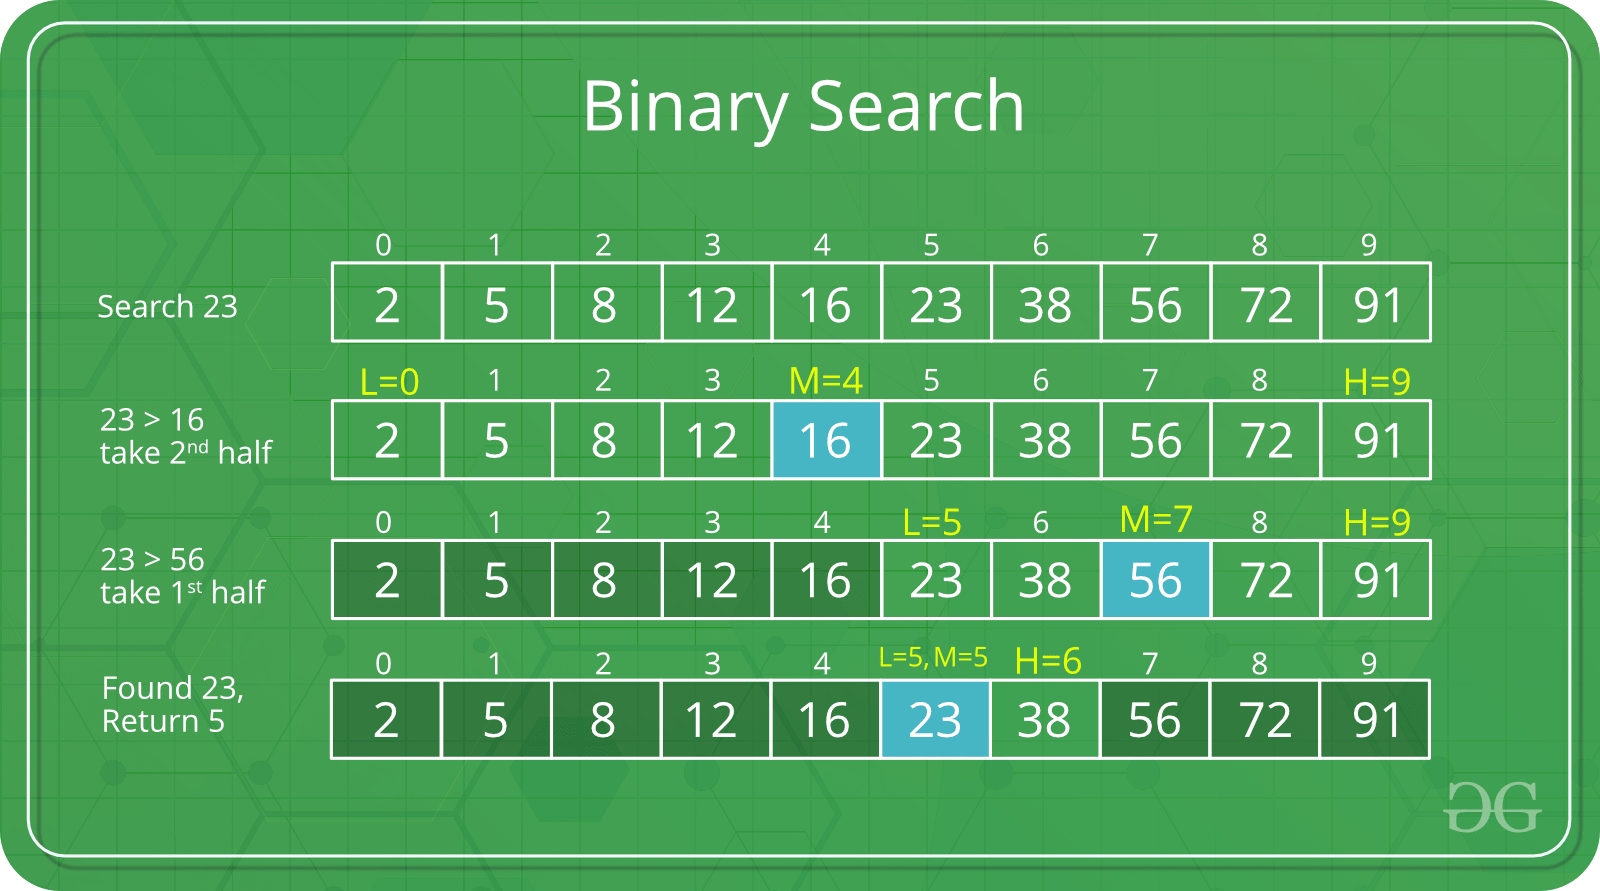
\includegraphics[width=\columnwidth, height=8cm]{Binary-Search.png}\begin{center}\textbf{Figure 1:} Binary Search\end{center}


\paragraph{Advantages of Binary Search}
The Binary Search technique generally has following mentioned advantages over Brute Force Algorithms.\\\\
\textbf{Time Efficiency} This approach generally reduces the running time of the algorithm because the running time of algorithm based on Brute Force is in general high order in nature. But when we are using the approach based on Binary, this running time generally decreases and becomes logarithmic in nature. This is because the approach of Binary Search keeps on dividing our range by 2 which makes it logarithmic in nature.\\
\textbf{Space Efficiency:} Space complexity is way less here, we only use O(1) space. Binary Search doesn't use much space, it just compares the target value to our middle element then reduces the range.\\\\
Note : We also have used a separate function in our case to count the number of trailing zeroes of a particular number, which would take O(log(n)), each time we run our Binary search, So, our final time complexity would be O(log(n)log(n)).However, space complexity still remains O(1).
\\\\\\\\This report further contains:
\begin{itemize}
\item 	Algorithm  Designs
\item 	Algorithm  Analysis
\item 	Experimental Study and Profiling
\item 	Conclusion
\item 	References
\item 	Appendix
\end{itemize}

\section*{ALGORITHM DESIGN}
A general problem based on the binary search somewhat like divide and conquer, but here we rather decrease and conquer. In other words, we divide our range into its half, then try to reach our answer. So our problem is no exception.

\paragraph{Algorithmic Steps:}

Our approach is we initially consider a range of 1 to 5n (we take our upper range initially to be 5n, because we are sure than we will find n or more zeros uptill 5n factorial, the we check for the middle number in our range, if the middle number has less than n zero then we update our lower range to middle+1, else we just update our upper range to middle-1, and store the current middle in a variable. Basically, we are finding the least number with n or more trailing zeros in its factorial.
\begin{enumerate}

\item	Input the number n.
\item	Create a function distance which will calculate the number of trailing zeroes in factorial of n.
\item   Create a variable, lets call it a.
\item	Implement Binary search, initially lo=1,hi=5*n.
\item	Count the number of trailing zeroes in mid, if it is less than n update lo=mid+1, else update hi=mid-1 and store mid in 'a'(a=mid).
\item	Finally check if number of trailing zeroes in factorial of a has exactly n zeroes or not, if it has print 'a' along with next 4 numbers(because a range of 5 numbers will always have equal trailing zeroes, as we are not multiplying extra '5' in that range (for trailing zeroes we need factor of 10=2*5, but in factorial the power of 2 will always be more than 5, so we just have to count for 5), otherwise if trailing zeroes in factorial of 'a' is more than n, we print that there doesn't exist any integer whose factorial has exactly n trailing zeros.
\\\\\\\\\\
\end{enumerate}

\lstset { %
    language=C++,
    backgroundcolor=\color{black!5},
    basicstyle=\footnotesize,
}

\begin{lstlisting}

int:
Function trailingZeroes(n)
    int cnt = 0; 
    while (n > 0):
        n /= 5; 
        cnt += n; 
        
    return cnt; 

Int:
Function main()
    int n
    Input n
    lo=1,hi=5*n,a=0
    
    while(hi>=lo):
        mid=(hi+lo)/2
        if(trailingZeroes(mid)>=n):
            a=mid
            hi=mid-1
        else
            lo=mid+1
    
    if(trailingZeroes(a)==n):
        print a,a+1,a+2,a+3,a+4
    else
        print The required number doesn't exist


\end{lstlisting}
    

	
\section*{ALGORITHM ANALYSIS} 
	
APRIORI ANALYSIS: Let T(n) and S(n) is the time and space respectively with input parameters defined above.

\paragraph{TIME COMPLEXITY DERIVATION:} Let Time complexity of above algorithm be T(n). Let us assume that we take O(logn) time in the Function trailingZeroes. The above algorithm divides the current range into half, so intuitively we can see than our algorithm with run for O(logn) time, with multiplication O(logn), so T(n) = O(log(n)log(n)) So T(n) can be expressed as follows:\\

\textbf{TIME COMPLEXITY DERIVATION:}
\rule{9cm}{1pt}
\textit{
T(n) = T(n/2) + log(n) if(n!=0) else T(n)=0\\
Using above relation, we get for T/2, T/8 etc as:\\
T(n/2) = T(n/4) + log(n)\\
T(n/4) = T(n/8) + log(n)\\
T(n/8) = T(n/16) + log(n) and so on……\\
.\\
.\\
.\\
.\\
Thus on combining we get the overall time 
complexity as:T(n) = T(log(n)log(n))\\}
\rule{9cm}{1pt}\\\\\\\\\\\\\paragraph{DIFFERENT CASES:} Now let us consider our algorithm in different 
scenarios.\\\\\textbf{BEST CASE/AVERAGE CASE/WORST CASE:} The time and space complexity of our approach approach in all the three cases is same , i.e, Time Complexity is  O(log(n)log(n)), as we are always dividing the range into half, in any case. Space complexity is the O(1) because we need are using constant space in each case.

\section*{PROFILING}

So, after the above analysis, let us have the glimpse of space and time graph and then comparison between both the approaches as a follow-up.

\paragraph{TIME ANALYSIS:}Following is the graph representing the time complexity of the algorithm.\\\\\\
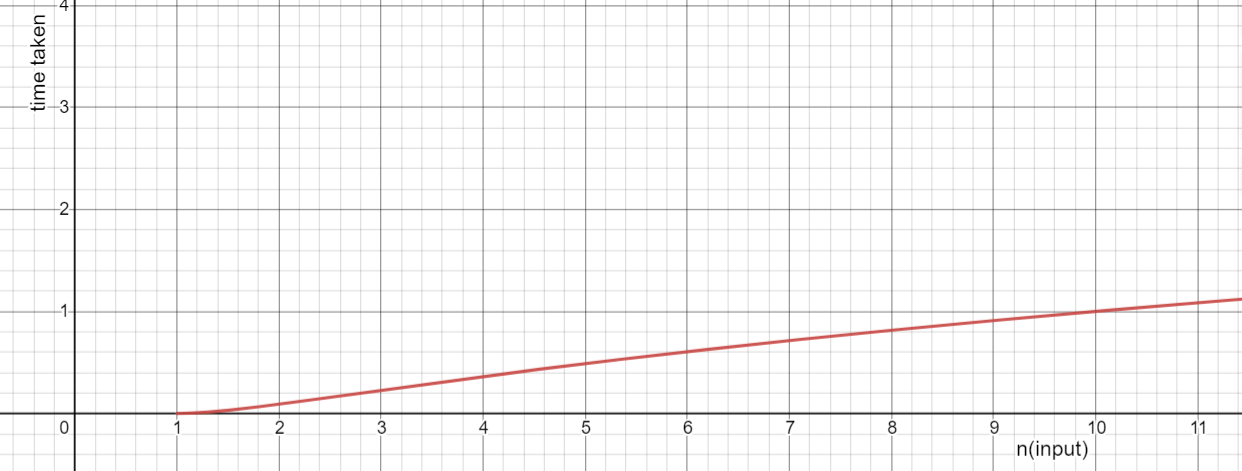
\includegraphics[width=\columnwidth, height=8cm]{Time Complexity.png}\begin{center}\textbf{Figure 2:} Time Complexity Graph\end{center}By the experimental analysis, we found that the more is the value of n, the more time it takes.

\paragraph{SPACE ANALYSIS:}Following is the graph representing the space complexity of the algorithm.\\\\\\
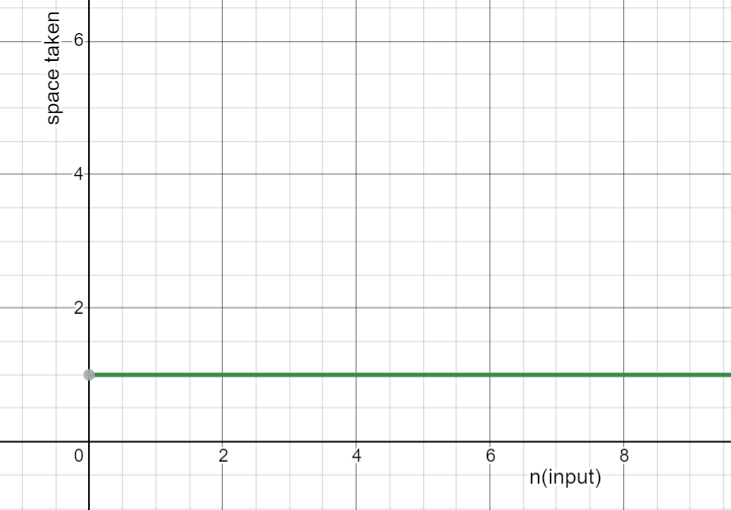
\includegraphics[width=\columnwidth, height=8cm]{Space Complexity.png}\begin{center}\textbf{Figure 3:} Space Complexity Graph\end{center}By the experimental analysis, we found that in any case, space taken is constant.
\newpage
\section*{APPLICATIONS}
Divide and Conquer is a wide variety of algorithmic paradigmn which beleives on the strategy of dividing the task and then applying an internal mechanism or algorithm in order to get the required answer. This programming paradigmn has several predefined algorithms which work on the basis of Divide and Conquer approach. Some of the applications of the Divide and Conquer Approach are:

\begin{enumerate}
\item \textbf{Binary Search:} It is a powerful programming algorithm based on the divide and conquer paradigmn which works very efficiently and gives answer in generally time cost, which is in general logarithmic in nature. (We used this in our question).
\item \textbf{Segment Trees:} It is another data structure which uses three standard operations:insert,query and update. All these three operations are based on divide and conquer because for example for building a segment tree, we first need to create in a recursive bottom up divide and conquer based technique.
\item  \textbf{Strassen’s Algorithm:} It is an efficient algorithm to multiply two matrices. A simple method to multiply two matrices need 3 nested loops. Strassen’s algorithm multiplies two matrices in efficient time.
\item \textbf{Quick Sort:} It is a sorting algorithm. The algorithm picks a pivot element, rearranges the array elements in such a way that all elements smaller than the picked pivot element move to left side of pivot, and all greater elements move to right side. Finally, the algorithm recursively sorts the subarrays on left and right of pivot element.
\item \textbf{Merge Sort:} is also a sorting algorithm. The algorithm divides the array in two halves, recursively sorts them and finally merges the two sorted halves.
\end{enumerate}
\section*{CONCLUSION}

So, with the above mentioned algorithms and their profiling, we come to the conclusion that this problem of finding the number of integers with trailing zeroes equal to n is achieving its best time complexity of O((logn)(logn)) and space complexity of O(1).\\\\ Also, binary search (or a part of divide and conquer) proved to be the most efficient algorithm here.

\section*{ACKNOWLEDGMENT}

We are very much grateful to our Course instructor Dr Mohammed Javed and our mentor, Md Meraz, who have provided the great opportunity to do this wonderful work on the subject of Data Structure and Algorithm Analysis specifically on the programming paradigm of Divide and Conquer.

\section*{REFERENCES}

\begin{enumerate}
\item Introduction to Divide and Conquer Technique:\\
https://www.geeksforgeeks.org/divide-and-conquer-algorithm-introduction/
\item Introduction to Algorithms by Cormen,Charles, Rivest and Stein.\\
https://web.ist.utl.pt/~fabio.ferreira/material/asa
\end{enumerate}
\end{multicols*}

\newpage
\section*{APPENDIX}
\textbf{To run the code, follow the following procedure:}\\
\begin{enumerate}
    \item Download the code(or project zip file) from the github repository.
    \item Extract the zip file downloaded above.
    \item Open the code with any IDE like Sublime Text, VS Code, Atom or some online compilers like GDB.
    \item If required, save the code with your own desirable name and extension is .cpp
    \item Run the code following the proper running commands(vary from IDE to IDE)
    \begin{enumerate}
        \item \textbf{For VS Code:} Press Function+F6 key and provide the input on the terminal.
        \item \textbf{For Sublime Text:} Click on the Run button and provide the input.\\
    \end{enumerate}
\end{enumerate}
\textbf{Code for Implementation is:}
\lstset { %
    language=C++,
    backgroundcolor=\color{black!5},
    basicstyle=\footnotesize,
}

\begin{lstlisting}
#include<bits/stdc++.h>
using namespace std;
int trailingZeroes(int n){ 
    int cnt = 0; 
    while (n > 0) { 
        n /= 5; 
        cnt += n; 
    } 
    return cnt; 
} 
int main(){
    int n;
    cin>>n;
    int lo=1,hi=5*n;
    int a=-1;
    while(hi>=lo){
        int mid=(hi+lo)/2;
        if(trailingZeroes(mid)>=n){
            a=mid;
            hi=mid-1;
        }
        else
            lo=mid+1;
    }
    if(trailingZeroes(a)==n){
        cout<<"The numbers whose factorial has "<<n<<" trailing zeroes are : ";
        for(int i=a;i<a+5;i++)
            cout<<i<<' ';
    }
    else{
        cout<<"No such number exists whose factorial has "<<n<<" trailing zeroes";
    }
}
\end{lstlisting}
\clearpage

	
\end{document}